\documentclass[a4paper,12pt]{report}
\usepackage{cmap} % Поиск PDF
\usepackage[T2A]{fontenc}  % Кодировка
\usepackage[utf8]{inputenc}  % Кодировка исходного текста 
\usepackage[english,russian]{babel}  % Кодировка исходного текста 
\usepackage{fontspec}
\usepackage{xcolor}
\usepackage{hyperref}
\definecolor{linkcolor}{HTML}{2d7ac7} % цвет ссылок
\definecolor{urlcolor}{HTML}{2d7ac7} % цвет гиперссылок
\usepackage{graphicx}
\graphicspath{ {./images/} }

\newcommand{\contractAddress}{0x37d29cb7d543300063a50d85389d409c01da7945}

\hypersetup{pdfstartview=FitH,  linkcolor=linkcolor,urlcolor=urlcolor, colorlinks=true}

\setmainfont{Ubuntu}
\providecommand{\versionnumber}{1.0}

% Title Page
\title{
\includegraphics[width=14cm]{logo}\\[2cm]Инфраструктура Portal Energy \\\normalsize v\versionnumber}
\author{Иванцов М. Мовчан П. Прусов М. Бутаков С. Патрикеев Б.}

\date{\today}


\begin{document}%
\maketitle
\tableofcontents
\clearpage


\chapter{Вступление}

Portal Energy была основана на слиянии технологий в сфере электроники, Big data, Blockchain. Стараясь приблизить экологичное будущее, мы, начиная с 2016 года, работали над созданием недорогих и универсальных зарядных устройств для электромобилей, понимая их необходимость для нашей страны и человечества уже в ближайшее время. На тот момент, мы точно определили для себя путь, как производственной компании и ежемесячно набирались опыта от заказа к заказу. 

Понимая, что инфраструктура – это не просто отдельно стоящие станции, передающие электричество в электромобили, а целая экосистема, которая может значительно сократить расходы населения на энергоносители, оптимизировать работу электросетей, а также поспособствовать развитию новых индустрий и рынков, таких как возобновляемая энергетика, аккумулирование энергии и умные города, мы привлекаем в нашу команду специалистов из этих сфер.

Ниже в тексте мы будем использоваться различные технические термины. Их краткое разъяснение дано в глоссарии. Если они вам знакомы, можете сразу переходить к разделу \ref{chapter3}.


\chapter{Глоссарий}

\section{Смарт-контракт}
Смарт-контракты похожи на классические контракты, за исключением того, что третьей стороной является множество людей, которые проверяют контракт на его исполнение и результат этого выполнения у всех участников должен совпадать, только тогда он будет считаться верным. В контракте мы можем прописать любые условия, которые надо выполнить. Из-за того что его выполняют множество участников, то мы не можем себе позволить исполнять очень сложные контракты, т.к. они будут требовать больших вычислительных мощностей. За вычисление берется комиссия в валюте ether(в сети Ethereum). После выполнения контракта сохраняется его состояние в блокчейне,
и удалить эту информацию невозможно.

\section{Блокчейн}
Выстроенная по определённым правилам непрерывная последовательная цепочка блоков, содержащих информацию. Простыми словами это цепочка блоков, каждый из которых обладает меткой времени, ссылкой на предыдущий блок и хранится на разных компьютерах.

\section{Криптовалюта}
Зашифрованный не регулируемый цифровой актив, использующийся в качестве аналога валюты в обменных операциях. Криптовалюта не имеет физической формы, она существует только в электронной сети в виде данных. Единицей такой валюты является «coin» (в переводе на русский –«монета»). При этом монета защищена от подделки, так как монета представляет собой зашифрованную информацию, скопировать которую невозможно.

\section{Ethereum}
Платформа для создания децентрализованных онлайн-сервисов на базе блокчейна (децентрализованных приложений), работающих на базе умных контрактов. Реализована как единая децентрализованная виртуальная машина.

\section{Ether}
Обменная единица Ethereum называются эфиром (англ. ether). Эта единица может делится на дробные части. 1/1000 — finney, 1/106 — szabo, 1/1018 — wei. Этой единицей может владеть как обычный кошелек, так и смарт-контракт. Такими же свойствами обладает и токен POE.

\section{Токен}
Единица учёта, не являющаяся криптовалютой, предназначенная для представления цифрового баланса в некотором активе, иными словами выполняющая функцию «заменителя ценных бумаг» в цифровом мире. Токены представляют собой запись в регистре, распределенную в блокчейн-цепочке.

\section{Токен ERC20}
ERC (Ethereum Request for Comments) — это официальный протокол для внесения предложений по улучшению сети Ethereum; 20 – уникальный идентификационный номер предложения. Технические спецификации для токенов, выпускаемых на блокчейне Ethereum, были опубликованы в 2015 году. Токены, отвечающие этим спецификациям, известны как токены стандарта ERC-20 и фактически являются смарт-контрактами на блокчейне Ethereum. Стандарт ERC-20 определяет набор правил, которые должны быть
соблюдены для того, чтобы токен был принят и имел возможность взаимодействовать с другими токенами в сети. Сами токены представляют собой блокчейн-активы, которые могут иметь ценность, а также могут быть отправлены и получены как любая другая криптовалюта. 

Отличие токенов ERC-20 от других известных криптовалют, напри-
мер, биткоина или Litecoin, в том, что они привязаны к сети Ethereum, используют принятый внутри этой сети формат адресов и отправляются при помощи Ethereum-транзакций. Соответственно, транзакции с участием токенов ERC-20 можно прослеживать в обозревателе блоков.


\href{https://etherscan.io/address/\contractAddress}{Здесь} можно отследить движение всех наших токенов.

\section{Приватный Blockchain}
Все сети, такие как Bitcoin, Ethereum, EOS, являются публичными, т.к. любой анонимно может писать в эту сеть, из за чего пропускная способность сетей становится более ограничена, не всегда хочется публиковать какие то конфиденциальные данные в общую сеть, а также будет очень большая комиссия, если транзакция имеет тяжелый смарт контракт со сложной логикой, в общем мы имеем множество ограничений. Поэтому для бизнесса больше подходят приватные блокчейн системы, такие как Hyperledger Fabric, Hyperledger Sawtooth, Quorum и другие. За счет того что в сеть могут писать только авторизованные участники, которых мы все знаем. 

В результате мы имеем масштабируемую пропускную способность, отсутствие комиссий за транзакции. Единственные расходы которые несет бизнес - это на поддержку инфраструктуры, т.е. сервера и специалистов, которые занимаются поддержкой системы.

\section{Etherscan}
Сервис для просмотра статистики сети Ethereum. С помощью него Вы можете просматривать. Основная функция Etherscan — отслеживание проводимых переводов. С помощью него Вы можете проверить статус вашей операции, проверить адреса и получить прочую информацию  \href{https://etherscan.io/}{https://etherscan.io/}.


\chapter{Электромобили как технология}
\label{chapter3}
Мы уверены, что электромобили являются будущим автомобильной индустрии. Почему это так? 
В первую очередь, благодаря тому, что электродвигатель гораздо более эффективен, в сравнении с двигателем внутреннего сгорания (далее ДВС) (КПД электродвигателя 95-98\% против 38\% у ДВС). Что уже само по себе выливается в значительную экономию средств (заряжать электромобиль в 5-6 раз дешевле, чем обычный автомобиль, из расчета на 100 км). Плюс, электропривод экологичен, что для жителей мегаполисов крайне важно. Да и в целом, вопрос экологии становится всё более и более актуальным. 

Кроме того, электромобили значительно манёвреннее и безопаснее обычных автомобилей, в связи с конструктивными отличиями. И наконец, потенциал электромобиля только начинает раскрываться, в то время, когда потенциал авто с ДВС уже достиг своего предела. Например, систему автопилотирования можно полноценно реализовать только на электромобиле.

Однако возникает логичный вопрос - если электромобили лучше по большинству показателей, в разы дешевле в эксплуатации и зарядке, экологичны - почему тогда они массово не распространены в нашей стране? 

Тем самым мы пришли ко второму нашему вопросу:


\chapter{Почему нет массового развития инфраструктуры в России?}
Вопрос действительно хороший. Чтобы вразумительно на него ответить, давайте посмотрим на страны, где электротранспорт уже распространён широко. 

\section{Электромобили в мире}
Лучше всего дела с электромобилями обстоят в Китае. В поднебесной за 2019 год было зарегистрировано более 1.2 млн новых автомобилей, а всего их 3.8 млн. Таже на начало 2019 года в Китае официально зарегистрировано более 1 млн зарядных станций.

На втором месте идут США. Там за 2019 год официально прибавилось 330 тыс. электромобилей. Всего в штатах их более 1.5 млн. штук, при этом зарядных станций там на 2019 год было более 200 тыс. штук.

В Европе, на конец 2019 года, количество электромобилей приблизилось к 2 млн штук, при проданных за год 550 тыс. штук и увеличении продаж в 1.5 раза в начале 2020 года.
Более того, дальнейшее будущее электротранспорта в развитых странах поистине безоблачно. 

Взгляните на графики роста выпуска электромобилей. Эти показатели говорят сами за себя. Стоит отметить, что в эту статистику входят не только абсолютные электромобили, но и подзаряжаемые гибриды (plug-in hybrids), т.к. подавляющее большинство из них имеют достаточно ёмкие батареи и полноценно используют зарядную инфраструктуру.
После 2023 года доля таких гибридов сокращается в пользу электромобилей.

Цифрами в перевёрнутых треугольниках обозначены некоторые из событий, ускоряющих смену автопарка на планете с ДВС на электро, либо являющихся важными контрольными точками этих изменений.

\vspace*{1cm}
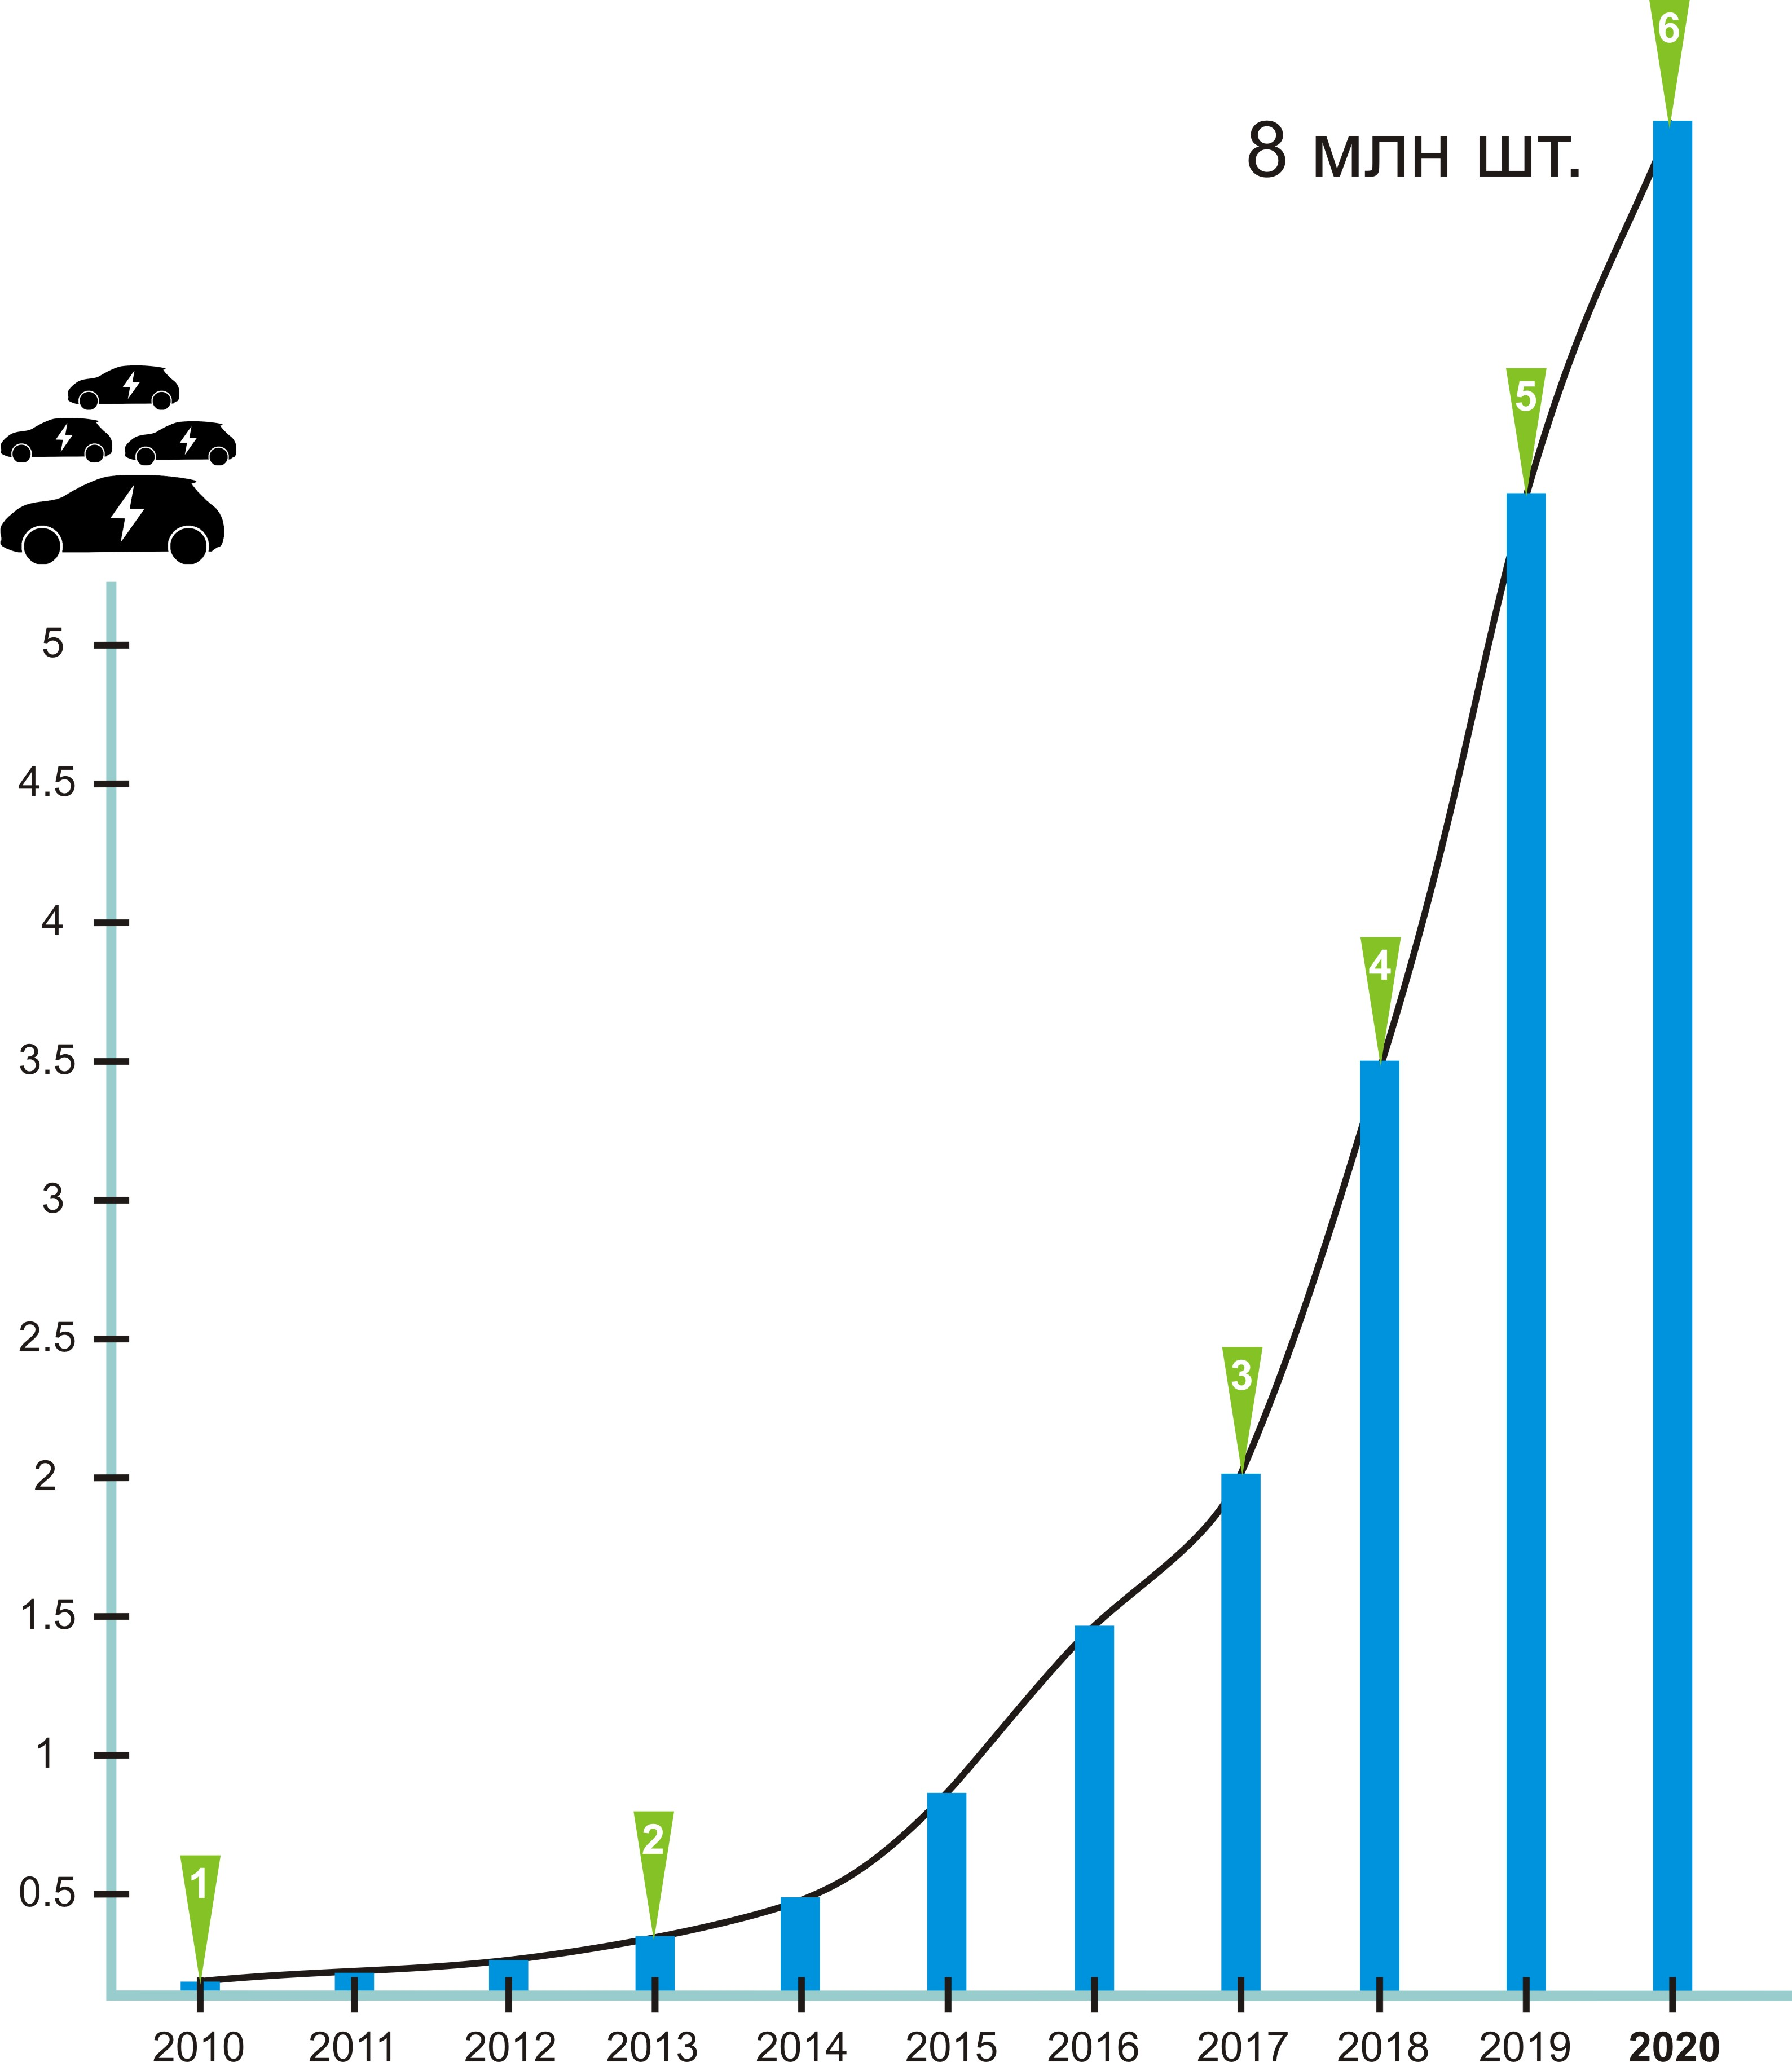
\includegraphics[width=12cm]{chart1}
\vspace*{1cm}

\begin{enumerate}
	\item Начало выпуска первого массового электромобиля в современной истории - Nissan Leaf
	\item Начало выпуска Tesla Model S
	\item Начало выпуска Tesla Model 3
	\item Каждый третий автомобиль в Норвегии электрический
	\item Количество зарядных станций в Европе превысило количество АЗС
	\item Количество проданных электромобилей Tesla превысило 1 млн штук
\end{enumerate}



\vspace*{1cm}
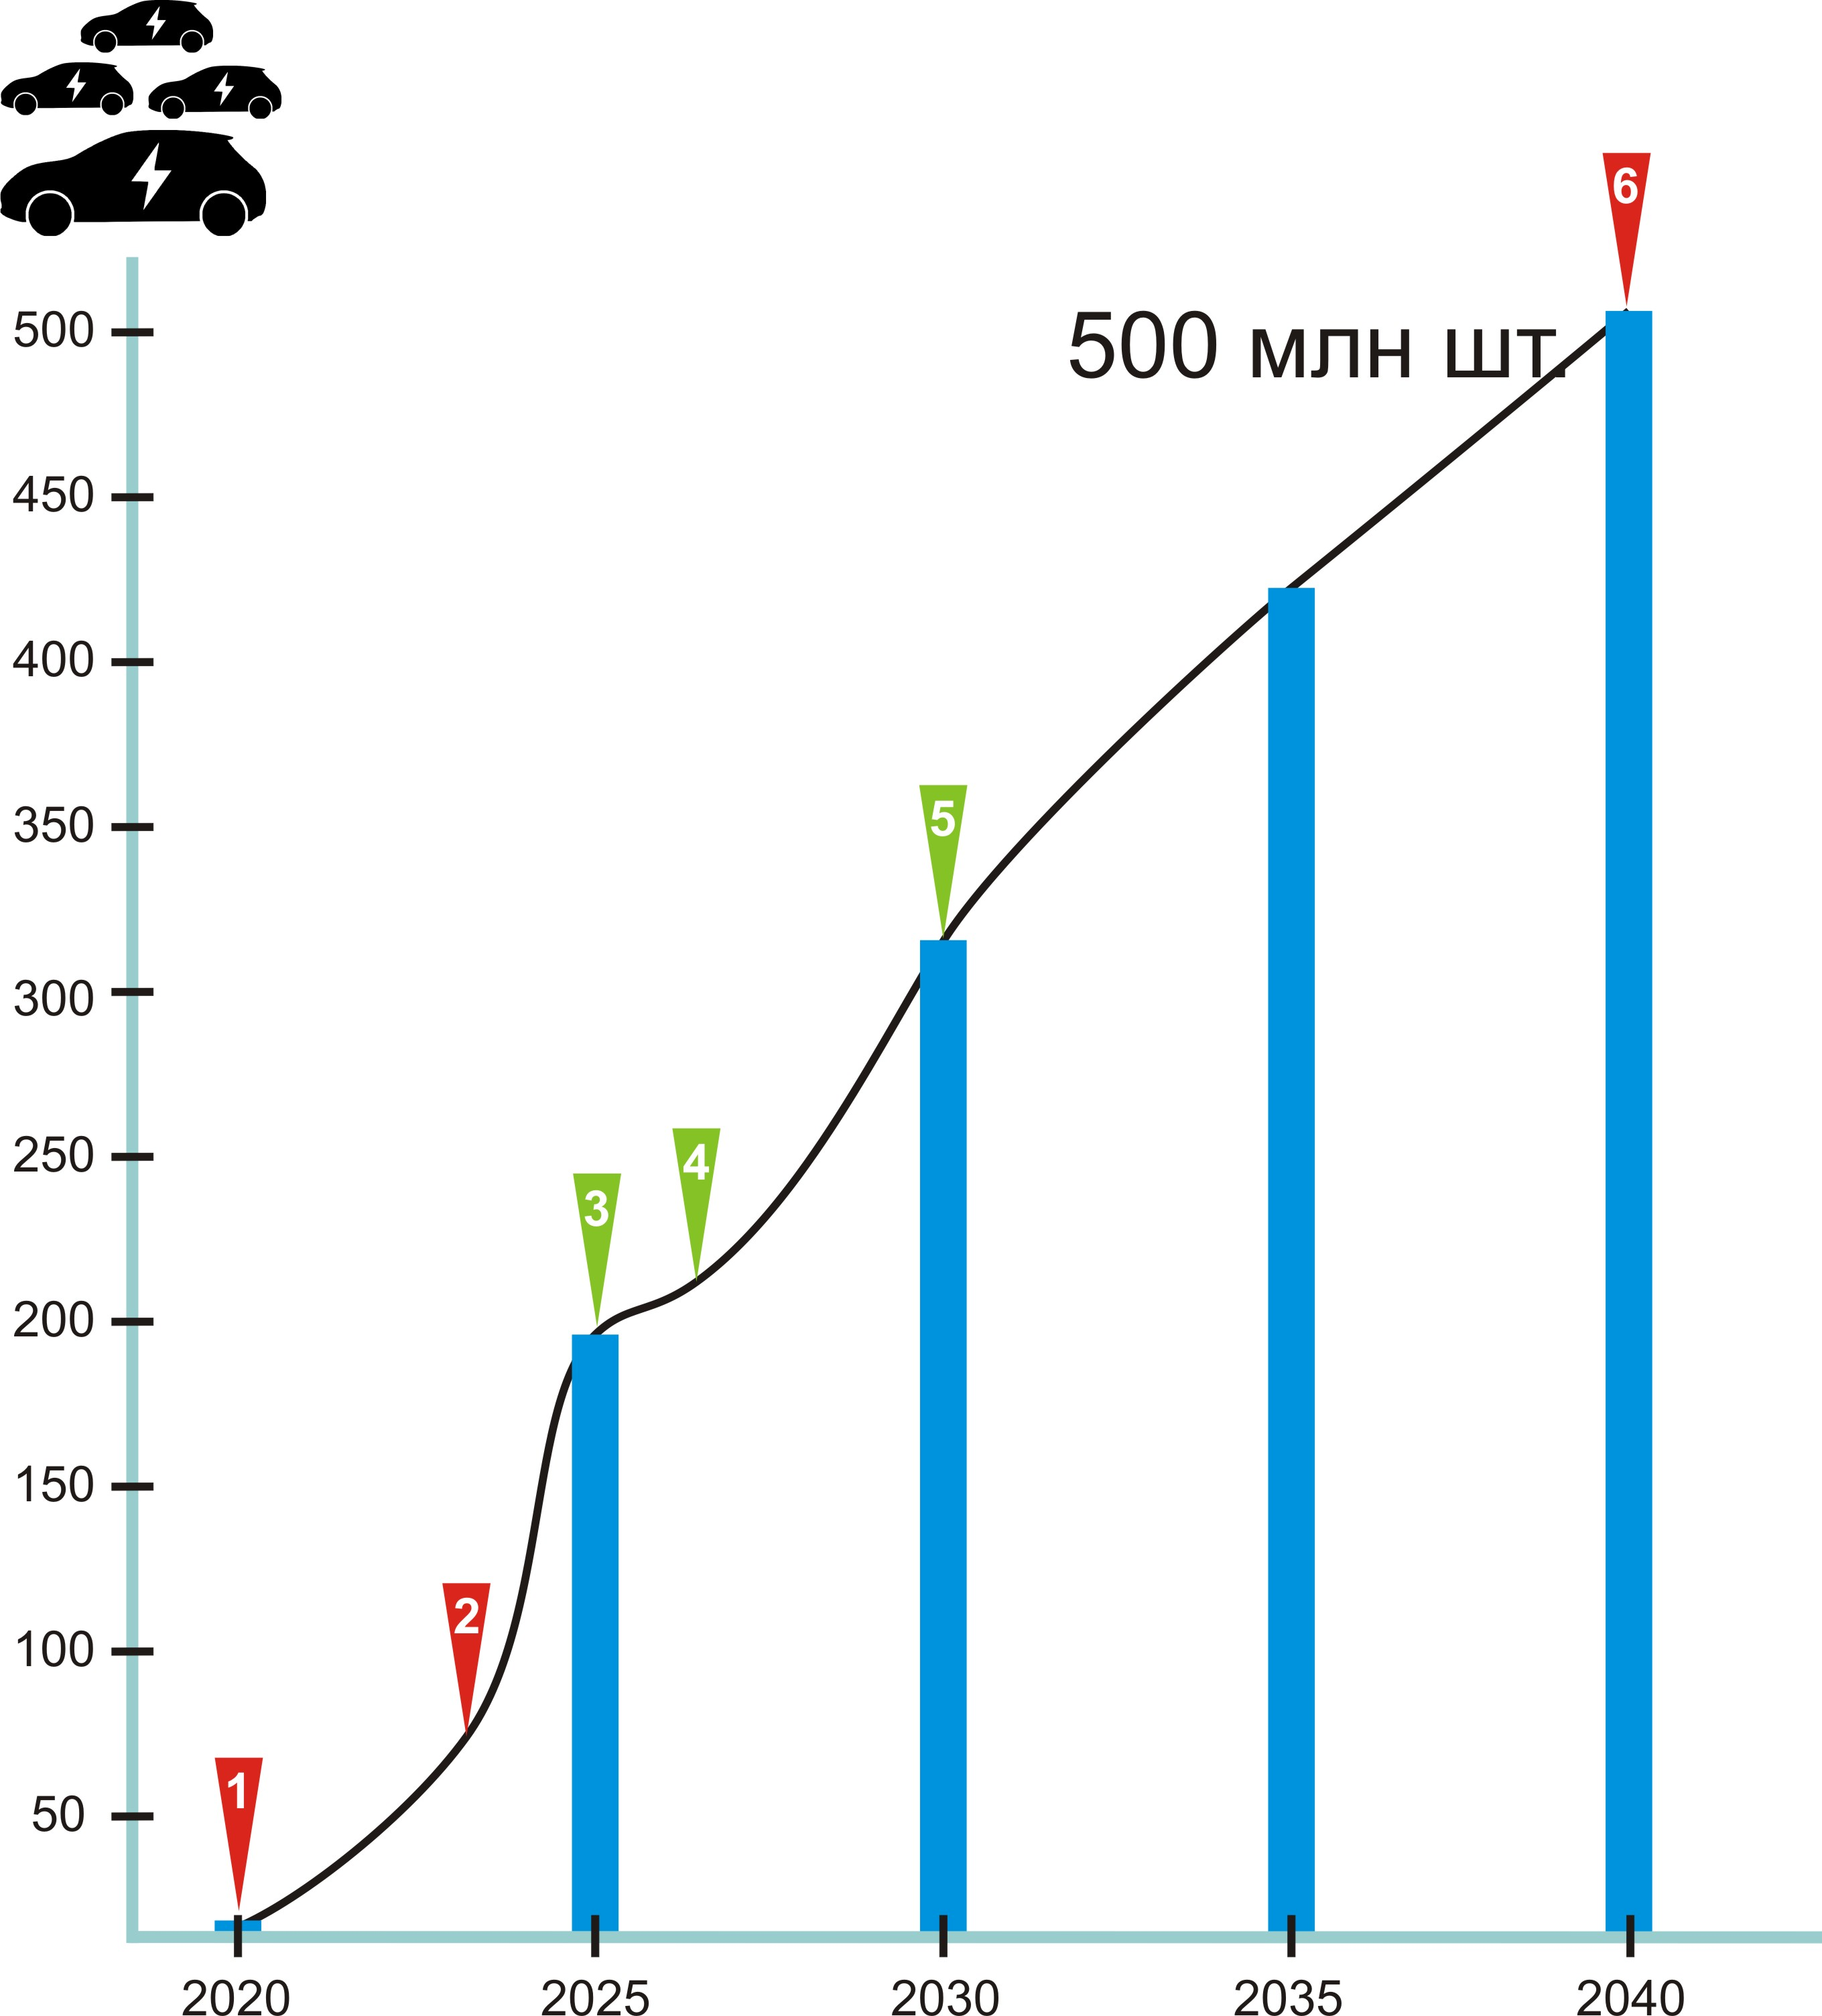
\includegraphics[width=12cm]{chart2}
\vspace*{1cm}

\begin{enumerate}
	\item Отказ от дальнейшей разработки в области ДВС крупнейших автопроизводителей, таких как BMW, Mercedes, Volvo, Audi, Volkswagen, Toyota
	\item Выравнивание стоимости электромобиля и автомобиля на ДВС (обусловлено снижением стоимости аккумуляторов)
	\item Начало распространения беспилотных, коммерческих электромобилей
	\item Toyota и Volkswagen прекращают выпуск автомобилей на ДВС
	\item Запрет эксплуатации ДВС в Голландии, Швеции, Шотландии, Дании и Израиле
	\item Полный запрет ДВС в Европе
\end{enumerate}


Какой вывод можно сделать из приведённых данных? Мы находимся на заре новой эры автотранспорта. Во всех развитых странах полным ходом идёт переход на электромобили, и это уже не просто фантазии отдельно взятых энтузиастов, это конкретные планы крупнейших автомобильных гигантов. 

Однако, светлое будущее не наступит само по себе. Его необходимо построить. 

\section{Электромобили в России}
Сейчас, например, в нашей стране на сегодняшний день всего около \textbf{500} полноценных зарядных станций. Чтобы понять, какое будущее ждёт электромобили при таком раскладе, нужно посмотреть на автомобили с ДВС через эту призму. Вы бы захотели приобретать авто, заправить которое можно было бы только в 500 точках на всю Россию? Которые, вдобавок, должным образом не обслуживаются, и внятных перспектив развития которых не предвидится. Наверное, нет. И это логично, поскольку автомобиль покупают не для самоистязания, а чтобы увеличить степень личной свободы и повысить комфорт передвижения. Поэтому неизбежным условием для увеличения количества электромобилей и их \textbf{комфортной} эксплуатации, является \textbf{развитие инфраструктуры}. 

\chapter{Проблематика инфраструктуры}
Помимо недостаточного количества самих станций, большинство из тех, что есть в нашей стране, расположены в самых странных и неудобных для автовладельца местах. А также не имеют должного обслуживания и адекватной информационной поддержки. В основном эти станции принадлежат гос. компаниям со всеми вытекающими.

Поэтому мы убеждены, что развитие электротранспорта в России должно начинаться с создания адекватной и удобной инфраструктуры. 
Именно такую задачу ставит перед собой компания Portal Energy.

\chapter{Мы - энтузиасты этой темы}
И хотим объединить других энтузиастов в России и по всему миру. Сейчас все надеются на то, что кто-то с большими финансами возьмёт и начнёт развивать инфраструктуру. В то время, как развивать ее можно уже сейчас, \textbf{сообществом}. 

Дополнительными стимулами для нас являются дизайн и урбанистика. Необходимо наполнять современные города действительно вдохновляющими предметами технического назначения, и для этой роли лучше всего подходят зарядные станции. Их конструктивным особенностям и дизайну мы придаем особое значение!

Наше производство находится в Санкт-Петербурге. Это цех металлообработки, пластико-формовочный цех и сборочная зона. Отдельно собирается и программируется вся электрическая начинка.

Мы убеждены, что в процессе создания зарядной инфраструктуры должен принимать участие широкий круг людей. Это обеспечит наилучшее качество, оптимальную цену станций и услуги подзарядки, а также поможет наиболее быстрому распространению электротранспорта в мире. Для этого разработана понятная \textbf{инвестиционная программа}.

Мы проектируем наши зарядные станции с учётом передовых технических возможностей и постоянно анализируем взаимодействие человека с инфраструктурой. Благодаря живому интересу к нашей деятельности, вокруг компании Portal Energy начинает расти сообщество современных людей, для которых важно будущее планеты, и на которое они могут непосредственно повлиять!

\chapter{План развития инфраструктуры}
Первое, что необходимо сделать - создать инструмент эффективного совместного взаимодействия. Portal Energy является таким инструментом. 

Дальше нужен производитель, который смог бы удовлетворить потребность будущей инфраструктуры в самих станциях и взять на себя задачи по их обслуживанию. Portal Energy является таким производителем.

Также немаловажным фактором при развитии инфраструктуры электротранспорта, является понимание его специфики. Модель поведения владельца электромобиля отличается от модели поведения владельца авто с ДВС. Местоположение АЗС обусловлено техническими ограничениями, поэтому они всегда находятся, в первую очередь там, где можно физически построить такую станцию и адекватно её обслуживать. Владелец авто с ДВС неизбежно привязан к локации заправки и для него это обязательная “боль” с которой он вынужден мириться. 

Что же касается зарядной станции для электромобиля, она может находиться там, где это реально будет удобно для автовладельца, потому как требования к пространству для установки станции незначительны. И, поэтому, при разработке карты местоположений станций, необходимо опираться в первую очередь на местоположение владельцев электротранспорта. И только в этом случае заправка автомобиля сможет перестать быть неизбежной головной болью владельца, а станет простым, понятным и не напряженным нюансом в эксплуатации автомобиля. Он будет заряжаться не где-то во время дороги, а пока владелец будет заниматься своими делами, поскольку в каждом удобном месте под рукой всегда будет зарядная станция.

В крупных городах наиболее рациональными местами для начала развития инфраструктуры являются торговые и бизнес центры, от которых будут тянуться нити зарядных станций ко всем районам. Между городами, расположенные через каждые 50-100 км станции постоянного тока, смогут полностью снять проблему подзарядки электромобиля в длительной поездке. 

Именно такой мы видим логику развития инфраструктуры.


\begin{center}
	\textbf{Вот основные вехи развития нашего проекта на ближайший год}
\end{center}

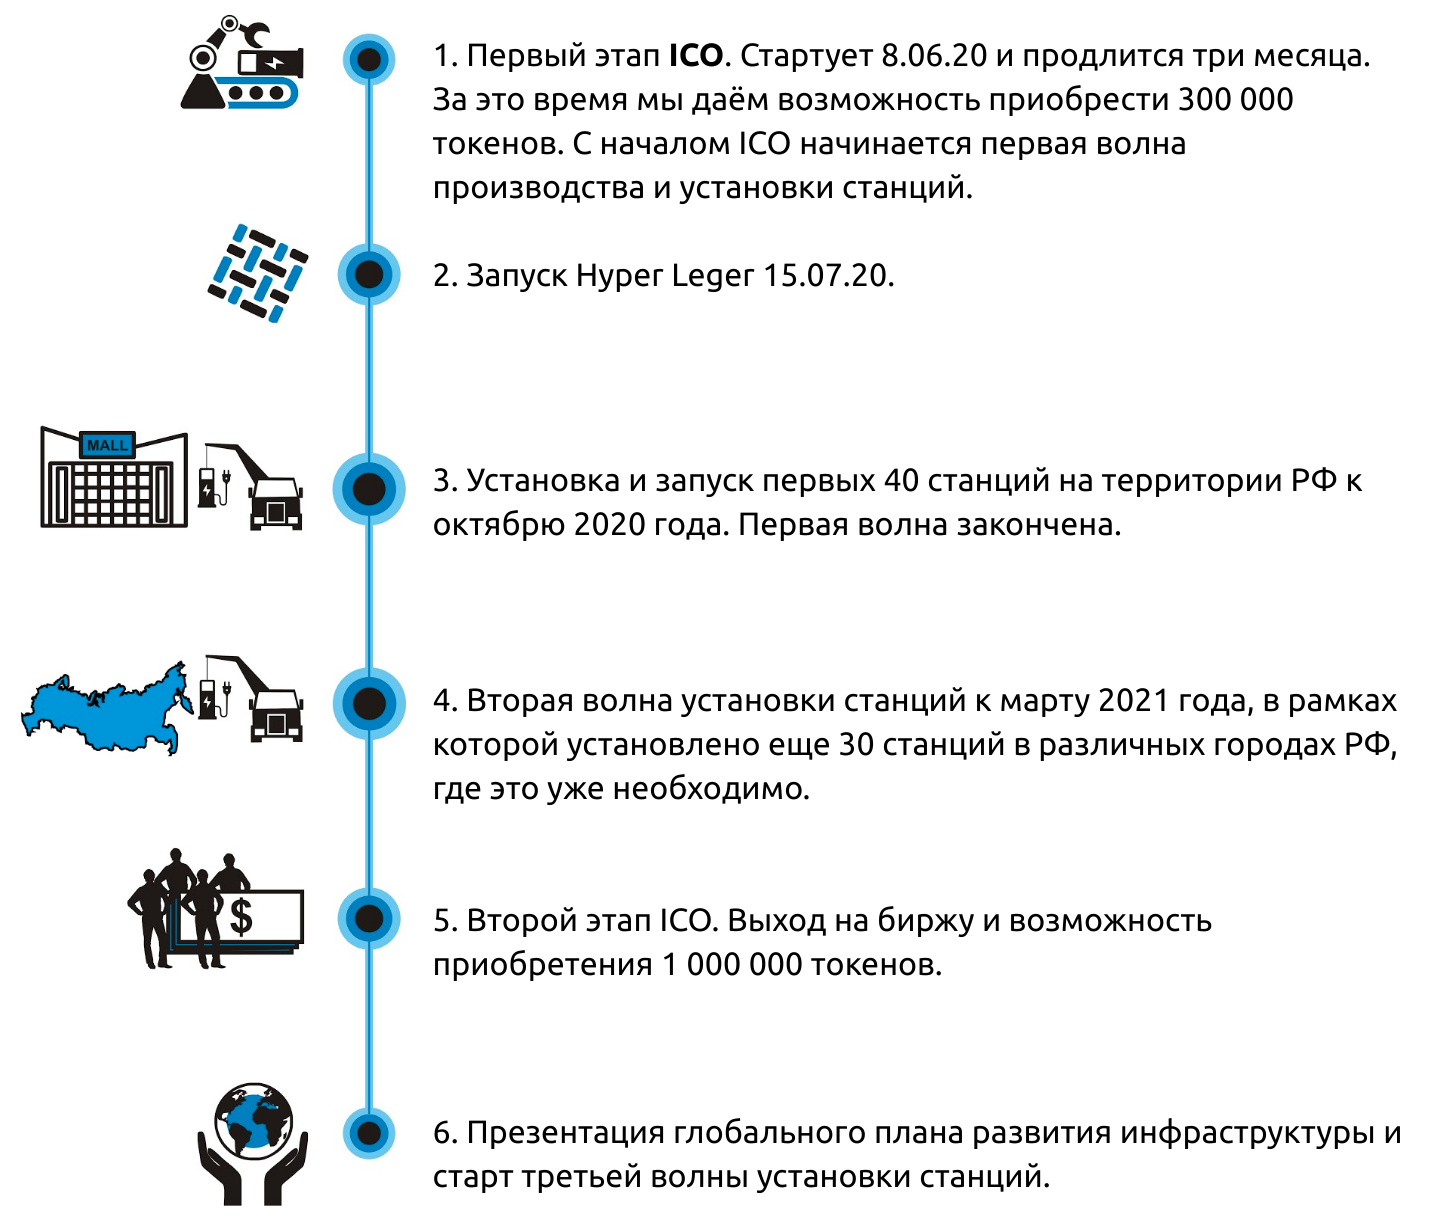
\includegraphics[width=13cm]{roadmap2}
\vspace*{1cm}

\chapter{Устройство компании}
Поскольку подобная задача может быть решена только в условиях абсолютного доверия участников сообщества друг к другу, мы обязаны были это доверие сформировать. По нашему мнению, лучшим фундаментом в формировании доверия является полная прозрачность всех финансовых процессов в организации. И для обеспечения такой прозрачности, мы выбрали \textbf{блокчейн}. 

Схема работы простая. Допустим стоимость одной станции составляет 4000 долларов. Купили токены 5 человек и покрыли эту сумму. Мы производим (по минимально возможной цене) и ставим эту станцию на парковку торгового центра, подключаем к сети. 
Далее весь доход от станции будет распределятся между участниками. При этом участники не привязаны к конкретной станции, а получают доход со всех установленных станций в системе, тем самым имея диверсифицированный портфель. Это позволит сгладить разницу между популярными и менее популярными локациями. 
Более подробно смотрите раздел \ref{capital} распределение дохода.

В итоге мы имеем инструмент который позволит более быстро и коллективно построить зарядную инфраструктуру с прозрачной и безопасной системой финансов.

\section{Токен}

Токен имеет адрес - \contractAddress
В нашей системе мы используем токены стандарта \textbf{ERC20}, которые называются \textbf{POE}. Основная их функция - выражать в цифровом формате зарядные станции, которые мы устанавливаем. Именно потому что они выражены материальными объектами, они имеют
определённую стоимость.

Приобретая токены, вы становитесь владельцем (собственником) части зарядной инфраструктуры. (Объём собственности соответствует вложенным средствам). В свою очередь, объекты инфраструктуры являются не просто физическими объектами, обладающим фактической стоимостью, в результате работы, они производят прибавочную стоимость, за счёт того, что люди используют их для удовлетворения своих потребностей, а именно зарядки автомобилей. В результате этого, в структуру будут постоянно поступать реальные деньги.

Мы используем блокчейн сеть Ethereum и стандарт токена ERC20, потому что данная сеть является крайне устойчивой и безопасной.
Для реализации токена мы использовали открытую разработку \\ (\href{https://openzeppelin.com/}{https://openzeppelin.com/}), которае прошла проверку на аудит безопасности многими крупными компаниями, что гарантирует безопасность нашего токена.


\subsection{Эмиссия и распределение токенов}

Токен имеет эмиссию в \textbf{10 000 000 POE}. Продаваться будет\textbf{ 5 000 000 POE}, остальные токены остаются за компанией. Это означает, что 50\% дохода с зарядных станций будет получать компания, это делается для того чтобы компания могла поддерживать текущую инфраструктуру в рабочем состоянии, а так же в будущем и дальше могла без привлечения дополнительных инвестиций развивать инфраструктуру, т.е. отношение зарядных станций к кол-ву токенов будет постоянно увеличиваться, и соответственно, доход с зарядных станций тоже. Как только система перестанет нуждаться в новых станциях, участники компании могут распродать свои токены сообществу, оставив только токены на обслуживание зарядной инфраструктуры.

\vspace*{0.5cm}

\includegraphics[width=13.6cm]{token-separate}
\vspace*{0.5cm}

\begin{itemize}
	\item A - 1 млн токенов которые распределяются между участниками компании до старта ICO, их участники могут использовать по своему усмотрению.
	\item B - 4 млн токенов хранится в multisig кошельке, прибыль с которого будет идти на развитие инфраструктуры.
	\item С - 5 млн токенов на multisig кошельке, с этого кошелька будут распределятся токены среди инвесторов 
\end{itemize}

\subsection{Распределение доходов с зарядных станций по токенам}
\label{capital}
Весь денежный учет будет производиться в блокчейн сети \textbf{Hyperledger Fabric}. 
Раз в период денежные средства будут переводиться в криптовалюту Ethereum на смарт-контракт PortalEnergyDistributor который отвечает за распределение средств по держателям токенов в нужном процентном соотношении.

Его математика простая, пример:

\begin{enumerate}
	\item Контракт получает на входе ether в размере 200 единиц.
	\item Получаем кол-во ether на каждый токен: 200/10000000 = 0,00002
	\item Получаем список держателей токенов
	\item По очереди берем каждого держателя токена, определяем кол-во токенов у держателя и умножаем на кол-во эфиров, т.е. Если адрес имеет 2000 токенов, то: 2000*0,00002 = 0,04 ether
\end{enumerate}

Периодичность будет изменяться от большего к меньшему в зависимости от накопленного капитала. В самом начале при запуске кол-во дохода будет небольшим и частое распределение не будет иметь смысла, т.к. комиссия за переводы будет составлять значительную часть самого дохода. С ростом дохода мы будем производить более частые выплаты, но не чаще чем 2 раза в месяц.


\section{Hyperledger Fabric}

\vspace*{0.5cm}

\includegraphics[width=13.6cm]{hyperledger-fabric}
\vspace*{0.5cm}


Помимо обеспечения безопасности, ключевым требованием к системе является финансовая прозрачность за пределами Ethereum сети.
Именно поэтому нами была выбрана Hyperledger Fabric.

Поскольку сеть Ethereum не позволяет экономно проводить большое количество транзакций, а также может быть временно нагружена и принимать транзакции долго и с динамической комиссией за транзакцию, что для нас неприемлемо, то для реализации бухгалтерии мы будем использовать стороннюю сеть, готовое решение для бизнеса - Hyperledger Fabric.

\textbf{Hyperledger Fabric} - это блокчейн платформа для создания приватных блокчейн сетей, которая позволит эффективно вести систему бухучёта для всей зарядной инфраструктуры, обладает высокой скоростью обработки транзакций, а также невозможностью подделать реестр.

Эту систему используют уже многие крупные компании:

\begin{itemize}
	\item Lamborghini - для сертификации своих автомобилей
	\item IBM - Для многих сфер своего бизнеса, в основном это связано
с сотрудниками и их учетом
	\item Walmart для учета и происхождения продуктов, взаимодействия с подрядчиками в рамках проекта IBM’s Food Trust
	\item и многие другие...
\end{itemize}

Еще одно \textbf{преимущество} приватной сети, в том, что мы можем давать разным ключам разные уровни доступа. Читать из сети смогут все, а писать в эту сеть смогут только зарядные станции которые имеют приватный ключ для подписи транзакции на оплату использованной энергии.

Также гиперледжер будет отвечать за функцию обмена фиатных денег, накопленных за определенный период в эфир. Он будет взаимодействовать с надежными биржами Binance, Bitfinex, Exmo, Bittrex и другие. Конвертация валюты в ether будет сразу происходить на контракт распределения Portal Energy Distribution.

Держатели от \textbf{5000} токенов получат возможность стать валидаторами транзакций в Hyperleger Fabric если они того пожелают, для того, чтобы система была еще более безопасной и устойчивой к внешнему вмешательству. Так же Hyperledger будет обладать копиями всех реальных документов которые будет заключать компания с другими организациями, например договор тарифного плана на электричество для кон-
кретной зарядной станции.
Каждый обладатель токена может запросить нотариально заверенную копию любого документа, заведенного в систему.


В заключение, мы хотим сказать, что прекрасно понимаем масштаб и сложность нашей цели, и понимаем, что нечто подобное можно реализовать только вместе. Сообщество единомышленников - это не какая-то абстрактная конструкция, это реальные люди, включая и тебя тоже. Поэтому, если ты готов принять непосредственное участие в изменении окружающей тебя действительности, вступай в сообщество Portal Energy.

\section{Присоединяйтесь}

\begin{itemize}
	\item Telegram канал - @portal\_energy
	\item \href{https://www.youtube.com/channel/UCtPxyCkz73i78F9HChlO61w}{Youtube}
	\item \href{https://www.instagram.com/petr_roadrunner/}{Instagram}
	\item \href{https://portalenergy.tech}{Сайт}
\end{itemize}

\textbf{По всем вопросам пишите в Telegram - @portal\_alexey}

\end{document}          
